\input{../Common/commands}

\begin{document}

\setlength\parskip{1ex}

\graphicspath{ {../Common/images/} }
\input{../Common/map}
\graphicspath{ {images/} }

% ----------------------------------------------------------------
% PAGE TITLE
% ----------------------------------------------------------------
\pgclrblue
\title{\headerpres{Data Analysis: \\ Data Preparation and Description}}
\author{\vspace{3cm} Technological University Dublin Tallaght Campus}
\date{Department of Computing}
\maketitle
\newpage

% ----------------------------------------------------------------
% PAGE DATA
% ----------------------------------------------------------------
\headerch{Data}
\begin{itemize}
\item Data can be structured or unstructured
\item Unstructured data is often transformed into structured data or can at least be abstracted as such
\item In this module, the term 'data' will be used as meaning 'structured data', unless indicated otherwise
\item Structured data can be shown in a table
\end{itemize}
\newpage

% ----------------------------------------------------------------
% PAGE DATA TABLE GENERAL 
% ----------------------------------------------------------------
\begin{center}
\headerss{Generalized data table}

\gendatatab
\end{center}
\newpage

% ----------------------------------------------------------------
% PAGE DATA TABLE GENERAL TERMINOLOGY
% ----------------------------------------------------------------
\headerch{Data table: terminology in statistics (S),\\ databases (DB) and machine learning (ML)} \\
\begin{tabular}{p{0.6\textwidth}|p{0.35\textwidth}|}
\cline{2-2}
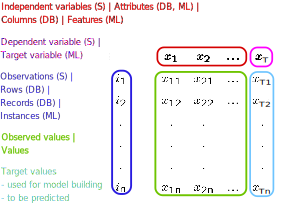
\includegraphics[width=0.6\textwidth]{table_general_terms.png}&\parbox[b][0.5\textwidth][t]{0.35\textwidth}{\vspace{-0.7ex} \footnotesize{'Independent' vs. 'dependent': Let's say we are looking at happiness. Respondents are asked to record how they feel every day for a year, because we are studying seasonal variations and the effect of sunlight on the feeling of happiness. The independent variables here are 'amount of sunlight' (which we can obtain from meteorological records) and 'time of year'. The dependent variable is 'happiness'. However, the two 'independent' variables are not really independent of each other (in the summer there is more sunlight). \emph{'Independent' in this context simply indicates the relationship with the 'dependent' variable}, which, by the same token, may be found not to depend on the 'independent' variables at all.}} \\
\cline{2-2} 
\end{tabular}
\newpage

% ----------------------------------------------------------------
% PAGE DATA VARIABLES
% ---------------------------------------------------------------2
\headerch{Variable types}
\begin{itemize}
\item \textbf{discrete} (e.g. natural numbers) or \textbf{continuous variables} (e.g. real numbers)
\item \textbf{categorical} or \textbf{numeric}
\item classification according to scale:
\begin{itemize}
\item \textbf{nominal scale}: categorical variable, no ordering among the possibe values (e.g. 'telecomms industry', 'pharmaceutical industry' etc.)
\item \textbf{ordinal scale}: categorical variable, values that can be ordered but without quantification of differences (e.g. low, medium and high)
\item \textbf{interval scale}: numeric variable, intervals between values can be compared but not ratios (e.g. temperature values $5^{\circ}$C, $10^{\circ}$C and $15^{\circ}$C)
\item \textbf{ratio scale}: numeric variable, both intervals and ratios between values can be calculated (e.g. prices \euro 5, \euro 10 and \euro 15)
\end{itemize}
\item dichotomous: the variable can take only two values and if the values are 0 and 1 the variable is referred to as \textit{binary} (e.g. 'customer has defaulted on their mortgage' or 'has not defaulted')
\item variables not used in analysis (e.g. customer id)
\end{itemize}
\newpage

% ----------------------------------------------------------------
% PAGE DATA TABLE PETS
% ----------------------------------------------------------------
\bgroup
\begin{center} 
{\bfseries \large Data table: pets for adoption} \\
\def\arraystretch{1.5}
\begin{tabular}{c c c c c c} 
\hline
\textbf{Name} & \textbf{Species} & \textbf{Breed} & \textbf{Gender} & \textbf{Age} & \textbf{Vaccinated} \\
\hline
Axel & Cat & Common & M & around 4 & NO \\
Baz & Dog & Lurcher & M & 2 & YES \\
Clodagh & Cat & Persian & F & 10 & YES \\
Dan & Cockatoo & N/A & M & 5 & ? \\
Emma & Dog & Staffie & F & 1.5 & YES \\
\hline
\end{tabular}
\end{center} 
\egroup
\newpage

% ----------------------------------------------------------------
% PAGE PREPARATION
% ---------------------------------------------------------------2
\headerch{Data preparation}
\begin{itemize}
\item Integration of data from multiple sources

\begin{itemize}
\item removal of duplicate entries
\item unit conversion
\item normalisation
\end{itemize}
\end{itemize}
\begin{howto}
  {\textbf{Min-max normalisation}}
  {Sometimes it is necessary to 'shift and rescale' a variable's data to a different range from the one they are originally provided in. This is typically done when a method requires normalised data, e.g. z-score for a hypothesis test, or when joining data sets that have the same variable specified on different scales (e.g. different units of measurement). The operation is called \textbf{min-max normalisation}. The formula to apply for each value is:
    $$x_{i(NEW)} = \dfrac{x_{i(OLD)} - x_{min(OLD)}}{x_{max(OLD)} - x_{min(OLD)}}(x_{max(NEW)} - x_{min(NEW)}) + x_{min(NEW)}$$

    \textbf{\color{darkgray}{Example:}}

    Let's say we have the set of values 2, 4, and 7 ($x_1=2$, $x_2=4$ and $x_3=7$) and are required to normalise it into the range 0-1, the new values would be:
    $$x_{1(NEW)} = \dfrac{2 - 2}{7 - 2}(1 - 0) + 0 = 0,\quad x_{2(NEW)} = \dfrac{4 - 2}{7 - 2}(1 - 0) + 0 = 0.4,\quad x_{3(NEW)} = \dfrac{7 - 2}{7 - 2}(1 - 0) + 0 = 1$$
    The new set is 0, 0.4 and 1.
    
    \tiny{\textbf{NOTES:}
    \vspace{-2ex}  
    \begin{itemize}
    \item When working with samples, the minimum and maximum values need to be those known for the population, rather than for the sample. Let's say we have data for exam marks given in percentages: 45, 67, 88 and 91. We know that the minimum and maximum in this case are 0 and 100 and we use those, rather than 45 and 91, for $x_{min(OLD)}$ and $x_{max(OLD)}$.
    \item The same technique can be used in any case where the scaling factor and a pair of corrsespondent source and target rangeg are known, even if no minimum and maximum don't exist. For example, converting temperatures from degrees celsius to farenheit involves a new 'minimum' of 32 and an old to new range mapping of 100 to 180: $temperature(^\circ F) = \dfrac{temperature(^\circ C)}{100}\times 180 + 32$
    \end{itemize}
    \vspace{0.5ex}
  }}{}{}
\end{howto}

\begin{itemize}
\item Cleaning

\begin{itemize}
\item resolution of ambiguities and errors (e.g abbreviations vs. full names or non-numeric values where numeric is expected, such as 'about 4')
\item removal or correction of invalid outliers, caused by:

\begin{itemize}
\item erroneous entry (typing error)
\item a mistake in measurement (e.g. a traffic counter reports a flow of 30 cars per second, which indicates a fault)
\item mixing of different measurement units (e.g. an adult's weight recorded as 55lbs may in fact be in kilograms)
\end{itemize} 

\item adjustments for time-dependent effects, such as inflation
\item removal of columns that are not relevant to the analysis (e.g. customer id or calibration information)
\item handling missing data:
  \begin{itemize}
  \item removal of observations
  \item imputation (ranging from simple replacement with the mean to complex methods such as multiple imputation)
    \end{itemize}
\item recording the steps of the cleaning process, so that if needed the information is available during future analyses
\end{itemize}
\end{itemize}
\newpage

%\further{Further reading on imputation of missing values in data} {
%http://www.stat.columbia.edu/~gelman/arm/missing.pdf

%https://www.theanalysisfactor.com/missing-data-criteria-for-choosing-an-effective-approach/

%http://www.statisticalhorizons.com/wp-content/uploads/MissingDataByML.pdf
%}
%\newpage

%----------------------------------------------------------------
% PAGE TABLE GENERAL ONE VAR
% ----------------------------------------------------------------
\pgclrgreen
\begin{center}
{\large The statistical data characterization concepts described in the remainer of this presentation all refer to a single data table column/variable/attribute} \\
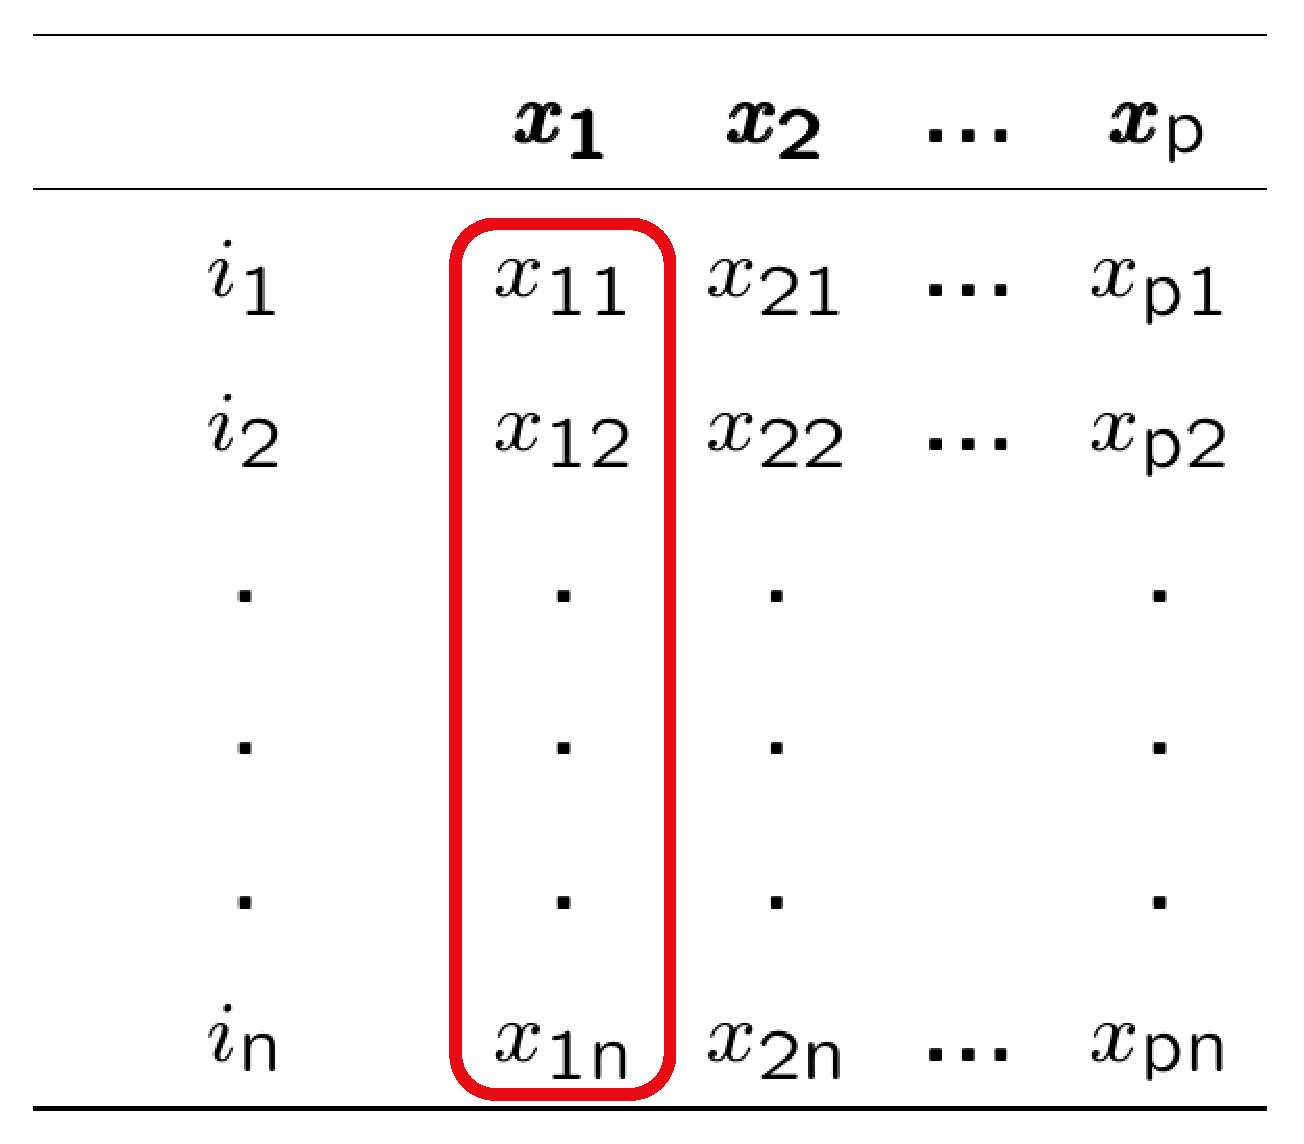
\includegraphics[width=0.5\textwidth]{table_general_one_var.eps} \\
\end{center}
\newpage

% ----------------------------------------------------------------
% PAGE STATISTICS SUMMARY DIAGRAMS AND TABLES
% ----------------------------------------------------------------
\headerch{Tally charts and frequency distributions} 

For datasets collected and/or processed manually
\begin{center}
\begin{tabular}{l@{\hskip 1cm}l}
\cline{2-2} 
\multirow{3}{*}{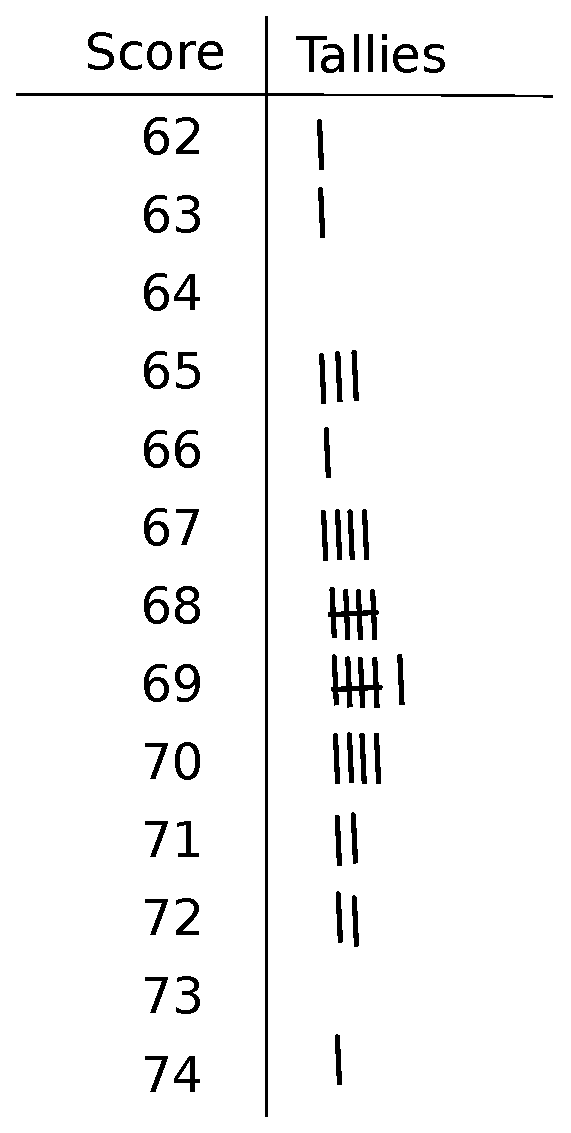
\includegraphics[width=0.2\textwidth]{stats_tallies.eps}} &   
\multicolumn{1}{|p{0.35\textwidth}|} {\footnotesize{[LEFT] Tally chart of the scores made in their final round by the 30 leading golfers in the 1992 Scottish Open}} \\
\cline{2-2} 
& \begin{tabular}{c|l}
\multicolumn{2}{c}{} \\
0 & 4, 7, 1, 0, 1, 6, 0, 1, 0 \\
1 & 2, 7, 0, 3, 0, 1, 4 \\
2 & 2, 6 \\
3 & 9 \\
4 &   \\
5 & 8 \\
\multicolumn{2}{c}{} \\
\end{tabular} \\
\cline{2-2} 
& \multicolumn{1}{|p{0.35\textwidth}|}{\footnotesize{[ABOVE] Results from a low-scoring cricket match, shown in a stem and leaf diagram. The stems are chosen so that there are up to about 10 of them, for clarity.}} \\
\cline{2-2}

\end{tabular}
\end{center}
\newpage

% ----------------------------------------------------------------
% CENTRAL TENDENCY
% ---------------------------------------------------------------
\headerch{Central Tendency}
\begin{itemize}
\item One of the most important way of summarising a variable is finding the centre of the values associated with it
\item There are three measures of central tendency: the \emph{mode}, the \emph{median} and the \emph{mean}. 
\begin{itemize}
\item The \textbf{mode} is the value that is most commonly reported for the variable. For example, if the following data were reported: \texttt{3, 4, 5, 6, 7, 7, 7, 8, 8, 9} then the mode would be \texttt{7}, as this is the most commonly occurring value in the set. If the set included an additional \texttt{8}, then the mode would be either \texttt{7, 8} or \texttt{7.5}. Always used with variables on a nominal scale, to which the other two measures of central tendency do not apply, but can be and is also used with variables measured on the other types of scale.
\item The \textbf{median} is the middle value in the set, when the set is ordered. For example, in the set \texttt{3, 4, 5, 6, 7, \textbf{7}, 8, 8, 8, 9, 9} the median is \texttt{7}, as this is the value with the same number of values on either side of it. If the number of values is even, the median is calculated as the average of the two middle values. For example, in the set \texttt{3, 4, 5, 6, 7, \textbf{7, 8}, 8, 8, 9, 9, 9} the median is \texttt{(7+8)/2=7.5}.
\item Finally, the \textbf{mean} is the average of the values and is calculated as:
$$\mean{x} = \dfrac{\mathlarger{\mathlarger{\sum}}_{\mathrm{i=1}}^{n} x_\mathrm{i}}{\mathrm{n}} $$
\end{itemize}
\end{itemize}

\newpage

% ----------------------------------------------------------------
% PAGE DISTRIBUTION
% ---------------------------------------------------------------
\headerch{ Distribution}
\begin{itemize}
\item Mode, median and mean provide a good initial idea of the data values but nothing about where in the range of possible values the set at hand actually is. 
\item A good place to start is a visual summary of the distribution, by way of bar charts and frequency histograms
\begin{itemize}
\item A bar chart simply displays the 'counts' for the different values of a variable: \par
  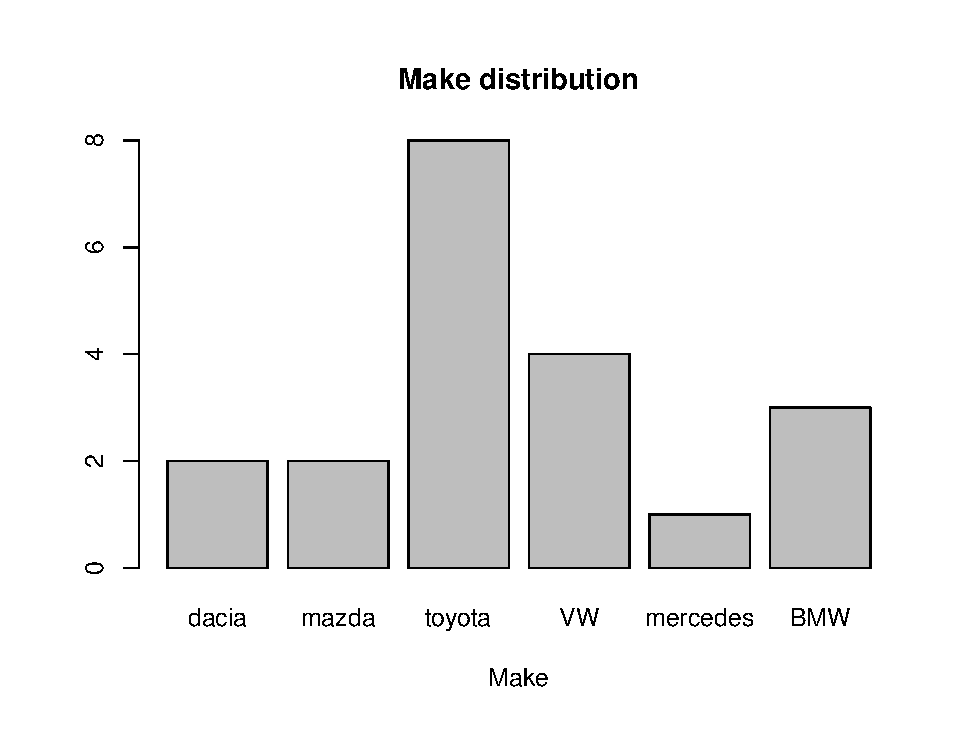
\includegraphics[width=0.5\textwidth]{barchart.eps} 
\item A \href{https://www.datacamp.com/community/tutorials/make-histogram-basic-r#gs.o8GxTqU}{frequency histogram} is useful for ordered variables with many values. It groups the values into ranges and gives an idea of the relative frequencies of the ranges.
\includegraphics[width=0.8\textwidth]{histograms.png}\\ [-1.5ex]
{\fontsize{10}{0}\selectfont \textbf{Source: [MSD]}}
\newpage
\item A probability density function (pdf) is a smooth function representing data in the same way as a histogram but based on a very large sample or theoretically derived. A very common probability density function is that for the \emph{normal distribution}, which can be expressed with the formula:
  $$f(x) = \dfrac{1}{\sqrt{2\pi\sigma^2}}e^{-\dfrac{(x-\mu)^2}{2\sigma^2}}$$
  where $\mu$ the mean and $\sigma$ the standard deviation.

    \includegraphics[width=0.4\textwidth]{normal_distrib_pdf.png}\\ [-1.5ex]
    {\fontsize{10}{0}\selectfont \textbf{Source: Wikipedia}}
\end{itemize}
\end{itemize}

\begin{howto}
  {Drawing a \textbf{histogram} from a frequency table manually}
  {
    The x-axis should show the ranges, while the area of the box above a range should be proportional to the frequency i.e. the number of values in that range. This proportionality is achieved when the height of the boxes corresponds to a \emph{frequency density} i.e. the number of values per some 'unit of range', which can be chosen arbitrarily. 

    \textbf{\color{darkgray} Example:}

    \begin{multicols}{2}
    The data to be displayed in a histogram is given in the following table:

    \begin{tabular}{c|c|c|c|c}
      \hline
      Range of values & 0-19 & 20-39 & 40-59 & 60-99\\
      \hline
      Frequency & 4 & 17 & 12 & 6\\
      \hline
    \end{tabular}

    The frequency density value shown in a histogram for a range can be expressed as:

    $FD = \dfrac{number\:of\:values\:in\:range}{\dfrac{width\:of\:range}{width\:of\:'unit\:of\:range'}}$

    For a range that has the same width as the 'unit of range' the frequency density is equal to the frequency. If we choose 20 for the 'unit of range', 3 out of the 4 ranges in the table will have 'unit of range' as their width and in those cases frequency density can be read directly from the table. For the fourth range, which has a width of 40, the frequency density value to be displayed in the histogram is $FD_4 = \dfrac{6}{\dfrac{40}{20}} = 3$. A sketch of the histogram derived in this way is shown below.

    \vspace{-1ex}
    \begin{center} \includegraphics[width=0.4\textwidth]{manual_histogram.png} \end{center}
  \end{multicols}
}
{}{\hspace{1ex}\vspace{-5ex}}
\end{howto}
\nopagebreak

\vspace{-5ex}
\begin{howto}
  {Drawing a \textbf{histogram} from a frequency table with R}
  {
    Frequency table data can be displayed in a boxplot, which is equivalent to the histogram for that data.

    \textbf{\color{darkgray} Example:}

    Using the same frequency table as above, we call the barplot function in R:

    {\fontsize{14}{16}\texttt{$>$ barplot(height=c(4,17,12,3),width=c(1,1,1,2),names=c(''0-19'',''20-39'',''40-59'',''60-99''))}}
    
    The height vector contains the calculated frequency densities, the width vector contains the widths of the ranges in 'units of range' and the names vector contains the range labels.
    \begin{center} \includegraphics[width=0.35\textwidth]{histogram_as_boxplot_r_example.png} \end{center}
  }
  {}{\hspace{1ex}\vspace{-4ex}}
\end{howto}
\nopagebreak

\vspace{-5ex}
\begin{howto}
  {Drawing a \textbf{histogram} from a dataset with R}
  {
    A function is available in R for drawing a histogram directly from a vector containing some attribute's values.

    \textbf{\color{darkgray} Example:}

    Let's 'make up' some data that fits the previous example. We feed the data into the R hist() function, with the resulting diagram equivalent to the one obtained from the frequency table.

    {\fontsize{14}{16}\texttt{$>$ hist(c(3,5,7,17,21,21,23,25,25,28,30,31,32,33,33,33,34,36,37,38,39,41,44,44,45,47,49,}
      \texttt{50,50,52,55,56,57,62,66,70,76,84,91),breaks=c(0,20,40,60,100))}}
    
    \begin{center} \includegraphics[width=0.35\textwidth]{histogram_r_example.png} \end{center}

    NOTE: The values on the y-axis are chosen so that the area under the entire histogram is equal to 1 (the 'unit of range' is 1/39, where 39 is the number of values in the set). However, the proportions remain the same as in the histogram created from the frequency table in the previous HOWTO panel.
  }
  {}{}
\end{howto}


  
\begin{itemize}
\item Distribution is also expressed through the measures of \emph{range} (the difference between the highest and the lowest value) and \emph{inter-quartile range} (the difference between the two values that lie (a) below the highest quarter of values and (b) above the lowest quarter of values, respectively)

\begin{itemize}
\item Box and whisker diagrams show the positions of the quartiles and the median in relation to the entire range. The vertical sides of the box are at the lower and upper quartile. The vertical line splitting the box is at the median. The leftmost and rightmost tips of the horizontal lines (the whiskers) are at the lowest and highest value in the range. \\ [0.5ex]
  Example: \\
  \includegraphics[width=0.6\textwidth]{BoxDiagramExample_c.jpg}\hspace{1ex} \parbox[t]{0.25\textwidth}{\vspace{-17ex}\tiny\emph{The box and whisker diagrams in this example show that Dickens' sentences are a lot longer (some over 200 words long!) than Archer's but also that Dickens produced a greater range of sentence lengths than Archer. }} \\ [-2ex]
   {\fontsize{10}{0}\selectfont \textbf{Source: [US]}}
\end{itemize}
\end{itemize}

\begin{howto}{Calculating the \textbf{range} of a dataset manually}{
  \begin{enumerate}
  \item order the data values by size
    
    \textbf{\color{darkgray} Example:} \texttt{2 3 4 4 5 5 5 7 9 10 10 11 12 12 15}

  \item the \emph{range} is the difference between the largest and the smallest value
    
    \vspace{3ex}\textbf{\color{darkgray} Example:}  \texttt{$range = 15 - 2 = 13$}
  \end{enumerate}}
{Finding the \textbf{range} of a dataset with R}{
  Use the following R command:
  
  \texttt{$>$ max(\emph{DATASET}) - min(\emph{DATASET})}

  \textbf{\color{darkgray} Example:}

  \texttt{$>$ dataset <- c(2, 3, 4, 4, 5, 5, 5, 7, 9, 10, 10, 11, 12, 12, 15)}

  \texttt{$>$ max(dataset) - min(dataset)}

  \texttt{[1] 13}

  The value given for the range by R is 13.}
\end{howto}
\begin{howto}{Calculating the \textbf{inter-quartile range (IQR)} manually}{
  \begin{enumerate}
  \item order the data values by size
    
    \textbf{\color{darkgray} Example 1 (odd number of  data values):}\texttt{ 2 3 4 4 5 5 5 7 9 10 10 11 12 12 15}

    \textbf{\color{darkgray} Example 2 (even number of  data values):} \texttt{2 3 4 4 5 5 5 7 9 10 10 11 12 12 15 16}

  \item identify the lower and upper half of the dataset (in the case of a dataset with an odd number of values, the median value is discarded)

    \textbf{\color{darkgray} Example 1:} \texttt{(2 3 4 4 5 5 5) \textbf{7} (9 10 10 11 12 12 15)}

    \textbf{\color{darkgray} Example 2:} \texttt{(2 3 4 4 5 5 5 7) (9 10 10 11 12 12 15 16)}

  \item the \emph{first quartile} or the \emph{lower quartile} or \emph{Q1} is equal to the median of the lower half of the dataset

    \textbf{\color{darkgray} Example 1:} \texttt{2 3 4 \textbf{4} 5 5 5, $Q1 = 4$}

    \textbf{\color{darkgray} Example 2:} 2 3 4 \texttt{\textbf{4 5} 5 5 7, $Q1 = \dfrac{4+5}{2}=4.5$}
    
  \item the \emph{third quartile} or the \emph{upper quartile} or \emph{Q3} is equal to the median of the lower half of the dataset

    \textbf{\color{darkgray} Example 1:} \texttt{9 10 10 \textbf{11} 12 12 15, $Q3 = 11$}

    \textbf{\color{darkgray} Example 2:} \texttt{9 10 10 \textbf{11 12} 12 15 16, $Q3 = \dfrac{11+12}{2}=11.5$}

  \item the \emph{inter-quartile range} or \emph{IQR} is the difference between the upper and lower quartiles

    \textbf{\color{darkgray} Example 1:} \texttt{$IQR = Q3 - Q1 = 11-4 = 7$}

    \textbf{\color{darkgray} Example 2:} \texttt{$IQR = Q3 - Q1 = 11.5-4.5= 7$}
  \end{enumerate}
  NOTE: The median of the data set is equal to the \emph{second quartile} or \emph{middle quartile} of the set.}{}{}
\end{howto}
\begin{howto}{Finding the \textbf{inter-quartile range (IQR)} with R}{
    \texttt{$>$ IQR(\emph{DATASET})}
    
    \textbf{\color{darkgray} Example:}

    \texttt{$>$ IQR(c(2, 3, 4, 4, 5, 5, 5, 7, 9, 10, 10, 11, 12, 12, 15))}

    \texttt{ [1] 6}

    NOTE: The value returned by R (6) differs from that calculated manually (7). This is because there are several methods for determining the IQR. All these are valid and the difference in results is not significant in the case of large datasets, which are the type that are encountered in real-life statistics.}{}{}
\end{howto}

  
\begin{itemize}
\item The \textbf{variance} describes the spread of the data and measures how much the values of a variable differ from the mean. When calculated with data across an entire population, the following formula is used:
  $$\sigma^2 = \dfrac{\sum_{\mathrm{i=1}}^{n} (x_\mathrm{i} - \mean{x})^2}{\mathrm{n}} $$
  where $\sigma^2$ is the variance, $n$ is the number of data values in the population, $x_i$ is the $i^{th}$ value and $\mean{x}$ is the mean value for the population.
  In the case that \emph{sample data} is used to estimate the variance of a population, the formula is:
  $$S^2 = \dfrac{\sum_{\mathrm{i=1}}^{n} (x_\mathrm{i} - \mean{x})^2}{\mathrm{n-1}} $$
  where $S^2$ is the exstimated variance, $n$ is the number of values in the sample, $x_i$ is the $i^{th}$ value and $\mean{x}$ is the mean value for the sample. Dividing by n when using sample data would consistently underestimate the population variance, essentially because the contribution of the difference between the estimated and population mean is always positive (owing to the squaring in the formula).
\item The \textbf{standard deviation} is the square root of the variance. Both the population and sample standard deviation are calculated as the square root of the respective variance:
$$\sigma = \sqrt{\dfrac{\sum\limits_{\mathrm{i=1}}^{n} (x_\mathrm{i} - \mean{x})^2}{\mathrm{n}}} \quad\quad\quad\quad S = \sqrt{\dfrac{\sum_{\mathrm{i=1}}^{n} (x_\mathrm{i} - \mean{x})^2}{\mathrm{n-1}}} $$
\newpage 
\end{itemize}


% ----------------------------------------------------------------
% page shape
% ---------------------------------------------------------------
\headerch{Frequency distribution shape}

The shape is represented with two measures, \textbf{skewness} and \textbf{kurtosis}.  
\begin{itemize}
\item \textbf{skewness} is a measure of imbalance in how the values of a distribution are placed to the left and the right of the mean. it can be calculated using the following formula:\\ [1ex]
\includegraphics[width=0.5\textwidth]{skewness_formula.png} \\ [-1.5ex]
     {\fontsize{10}{0}\selectfont \textbf{Source: [MSD]}}

two distributions, one with a positive and one with a negative skewness:\\ [1ex]
\includegraphics[width=0.55\textwidth]{skewness_picture.png} \\ [-1.5ex]
{\fontsize{10}{0}\selectfont \textbf{Source: [MSD]}}

there are many other ways of measuring skewness, such as the \textbf{quartile coefficient of skewness} or the \textbf{pearson's coefficient of skewness}

\item \textbf{kurtosis} is a measure of of the peak of the distribution and how close it is to the mean. kurtosis formula: \\[1ex]
\includegraphics[width=0.5\textwidth]{kurtosis_formula.png} \\ [-1.5ex]
     {\fontsize{10}{0}\selectfont \textbf{Source: [MSD]}}

two distributions, with different values for kurtosis:\\ [1ex]
\includegraphics[width=0.55\textwidth]{kurtosis_picture.png} \\ [-1.5ex]
     {\fontsize{10}{0}\selectfont \textbf{Source: [MSD]}}



\end{itemize}
\newpage

% ----------------------------------------------------------------
% CONFIDENCE INTERVALS
% ---------------------------------------------------------------
\headerch{Confidence interval}

The confidence interval is a measure of how well a property calculated on a data sample represents the same property with respect to the entire population.  
\begin{itemize}
\item  A confidence interval is expressed as a range of values within which a statistic will be found in a large  proportion of cases. This proportion is specified as a percentage, most often 95\%. For example, a confidence interval may be:
  $$ \mathbf{x = 455.5 \pm 5.4, \text{ with a confidence level of }  99\%} $$
\item Confidence intervals are calculated using \textbf{sampling distributions}. These can be distributions of various statistics, e.g. the sample mean. Like population distributions, sampling distributions have:
  \begin{itemize}
  \item a mean, called the \textbf{expected value}
  \item a standard deviation, called the \textbf{standard error}
  \item a distribution, called the \textbf{sampling distribution}
  \end{itemize}
\newpage
\item For an example, we look at the confidence interval for the mean of a distribution.
  \begin{itemize}
  \item The sampling distribution for a mean is a normal distribution as long as the samples contain more than 30 values, according to the \emph{law of large numbers} or the \emph{central limit theorem} (the sampling distribution for samples smaller than 30 is a \emph{Student's t-distribution} and a confidence interval can be defined for that case as well, but it is outside of the scope of the module) 
  \item The standard error of the sampling distribution is $\dfrac{s}{\sqrt{n}}$, where $s$ is the standard deviation of a sample and n is the size of the sample
  \item The following picture shows a z-distribution (a normal distribution with standard deviation 1 and mean 0):\\ [1ex]
    \includegraphics[width=0.6\textwidth]{confidence_int.png} \\ [-2ex]
    {\fontsize{10}{0}\selectfont \textbf{Source: [MSD]}}
    
    If we define $\alpha = 1-\dfrac{confidence\_level}{100}$, where $confidence\_level$ is the percentual value of the required or declared \emph{confidence level} (e.g. $95\%$), then the values on the x-axis of the z-distribution below and above which the area covered by the distribution is equal to $\alpha/2$ define the normalized \emph{confidence interval}. The two values, which we will name $-z_{\alpha/2}$ and $z_{\alpha/2}$, differ only in sign, since the z-distribution is symmetric with respect to the y-axis.
  \item The confidence interval is then: 
    $$\mean{x}\pm z_{\alpha/2}(\dfrac{s}{\sqrt{n}}), \text{ with a confidence of } confidence\_level$$
    The meaning of this statement is that there is a $confidence\_level$ level of confidence that the actual mean of the population lies somewhere in the interval spanning the width $z_{\alpha/2}(\dfrac{s}{\sqrt{n}})$ to either side of the value of the sample mean, $\mean{x}$.
    \item The value of $z_{\alpha/2}$ for a given confidence level percentage can be looked up from a z-distribution table
  \end{itemize}
\end{itemize}
\newpage
\includegraphics[width=0.8\textwidth]{1_1_8_z_distrib_pp.png}

\newpage


% ----------------------------------------------------------------
% HYPOTHESIS TESTS
% ---------------------------------------------------------------
\headerch{Hypothesis tests}

A hypothesis test is used to check if a sample of data supports a particular hypothesis made about the population from which the sample was drawn.
\begin{itemize}
\item A hypothesis test definition uses the same principle as confidence interval definition, i.e. works with an interval for a data statistic, which associated with a probability value
\item In the case of hypothesis testing, the probability used is the \emph{threshold of probability} or \emph{level of significance} (while in the case of confidence intervals the probability was the \emph{confidence level})
\item The interval in hypothesis testing is defined by between one or two critical values (while in the case of confidence intervals it was called the \emph{confidence interval})
\item A hypothesis test is stated through a null hypothesis and an alternative hypothesis and the null hypothesis is either accepted or rejected at the end of the test
\item For an example, let us look at the mean of a population once more. The hypotheses would be stated in this way:
{\setlength{\mathindent}{0cm}
\begin{align*}
  &H_0: \mu = 100    \quad \text{null hypothesis} \\
  &H_a: \mu \neq 100 \quad \text{alternative hypothesis} \\
\end{align*}}
  \begin{itemize}
  \item Let's assume a sample of more than 30 observations, which means that the sampling distribution is normal (see the section on confidence intervals)
  \item The standard error of the sampling distribution is $\dfrac{s}{\sqrt{n}}$, where $s$ is the standard deviation of a sample and n is the size of the sample
  \item Critical values are marked in a z-distribution (a normal distribution with standard deviation 1 and mean 0) so as to correspond to the test's level of significance. If the test is two-tailed, there are two critical values and if it single-tailed there is only one. In the picture below, critical values are shown for a two-tailed test with a level of significance of $5\%$ (the areas under the z-distribution curve outside of the range C1 to C2 add up to 0.05): \\ [1ex]
    \includegraphics[width=0.6\textwidth]{hypothesis_test.png} \\ [-1.5ex]
    {\fontsize{10}{0}\selectfont \textbf{Source: [MSD]}}
    
  \item The hypothesis test is accepted if the test value, calculated as follows, falls between C1 and C2:
    $$ T = \dfrac{\mean{x} - \mu_0}{s/\sqrt{n}}$$
    where $\mean{x}$ is the sample mean, $\mu_0$ is the hypothesised mean, $s$ is the standard deviation and $n$ the size of the sample.
    \item The critical values can be looked up for a given level of significance in a z-distribution table
  \end{itemize}
\item Two types of errors can occur with respect to the outcome of a hypothesis test:
  \begin{itemize}
  \item Type I error - when the null hypothesis is rejected even though it is true
  \item Type II error - when the null hypothesis is accepted even though it is not true
  \end{itemize}
\end{itemize}

\newpage

\headersec{References}
The pictures in this presentation were taken from the following books. The source for each picture is cited beside it. \\

\textbf{[DSB]} \emph{Data Science for Business: What you need to know about data mining and data-analytic thinking}, by Foster Provost and Tom Fawcett, O'Reilly Media, 2013. \\

\textbf{[MSD]} \emph{Making Sense of Data I: A Practical Guide to Exploratory Data Analysis and Data Mining}, by Glenn J. Myatt and Wayne P. Johnson, John Wiley \& Sons, 2014. \\

\textbf{[US]} Understanding Statistics, by Graham Upton and Ian Cook, Oxford University Press, 1996.


\end{document}
